\documentclass[pdflatex,compress,mathserif]{beamer}

%\usetheme[dark,framenumber,totalframenumber]{ElektroITK}
\usetheme[darktitle,framenumber,totalframenumber]{ElektroITK}

\usepackage[utf8]{inputenc}
\usepackage[T1]{fontenc}
\usepackage{lmodern}
\usepackage[bahasai]{babel}
\usepackage{amsmath}
\usepackage{amsfonts}
\usepackage{amssymb}
\usepackage{graphicx}
\usepackage{multicol}
\usepackage{lipsum}

\newcommand*{\Scale}[2][4]{\scalebox{#1}{$#2$}}%

\title{PEMODELAN JARINGAN KOMUNIKASI}
\subtitle{Ethernet Connection Media}

\author{Tim Dosen Pengampu}

\begin{document}

\maketitle

\begin{frame}
	\frametitle{Layer 1 – The Physical Layer}
	\begin{itemize}
		\item OSI Layer 1 conveys the bit stream - electrical impulse, light or radio signals - through the network at the electrical and mechanical level.
		\item It provides the hardware means of sending and receiving data, including defining cables, interface cards and physical aspects.
	\end{itemize}
\end{frame}

\begin{frame}
	\frametitle{Layer 1 Connection Types\\ for Ethernet - UTP}
	\begin{itemize}
		\item Ethernet LAN connections can be carried over coaxial cable (no longer used), twisted copper pair cable, fiber cable or wireless.
		\item Copper UTP (Unshielded Twisted Pair) cables are commonly used to connect desktop computers to switches.
		\item Connector type is RJ-45 and maximum length is 100 metres.
		\item Twisted pair \href{https://en.wikipedia.org/wiki/Twisted_pair}{\beamergotobutton{Link}}
	\end{itemize}
\end{frame}

\begin{frame}
	\frametitle{Straight-Through vs Crossover UTP Cable}
	\begin{itemize}
		\item The receive and transmit wires in a UTP cable can be wired to the RJ- 45 connector as either straight-through or crossover.
		\item Straight-through cables are used to connect an end device such as a PC or router to a switch.
		\item Crossover cables are used to connect devices together directly. They are most often used to connect two devices of the same type: e.g. two computers or two switches to each other.
		\item Modern switches support Auto MDI-X where the receive and transmit signals are reconfigured automatically to yield the expected result.
	\end{itemize}
\end{frame}

\begin{frame}
	\frametitle{Fiber Cables}
	\begin{itemize}
		\item Fiber optic cables can be used to support longer distances or higher bandwidth requirements.
		\item For example between separate buildings in a campus, or for switch to switch connections inside a building.
	\end{itemize}
	\begin{center}
		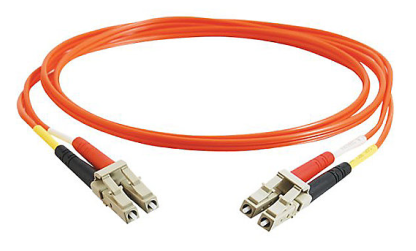
\includegraphics[width=0.6\linewidth]{img/img01}
	\end{center}
\end{frame}

\begin{frame}
	\frametitle{Single Mode vs Multi Mode Fiber}
	\begin{itemize}
		\item Single Mode or Multi Mode Fiber can be used.
		\item Single Mode supports higher bandwidth and longer distances but is more expensive.
		\item Multi-mode optical fiber \href{https://en.wikipedia.org/wiki/Multi-mode_optical_fiber}{\beamergotobutton{Link}} 
	\end{itemize}
\end{frame}

\begin{frame}
	\frametitle{Fiber Connectors}
	\begin{center}
		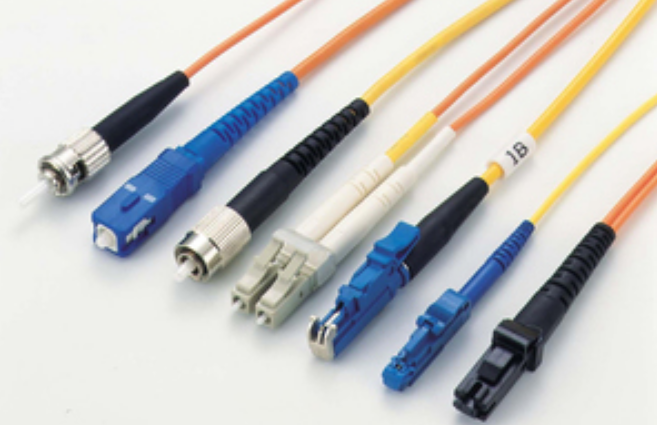
\includegraphics[width=0.6\linewidth]{img/img02}
	\end{center}
\end{frame}

\begin{frame}
	\frametitle{PoE Power over Ethernet}
	\begin{center}
		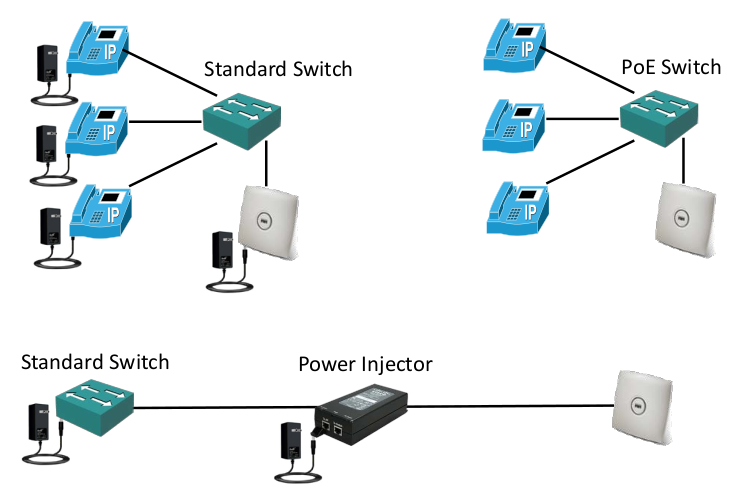
\includegraphics[width=\linewidth]{img/img03}
	\end{center}
\end{frame}


\end{document}
